\section{Methodology}


% Requires in preamble:
% \usepackage{tikz}
% \usetikzlibrary{positioning}

% Requires in preamble:
% \usepackage{tikz}
% \usetikzlibrary{positioning}

% \begin{figure*}[t]
% \centering
% \resizebox{\linewidth}{!}{%
% \begin{tikzpicture}[
%   font=\normalsize,
%   node distance=0.70cm and 1.05cm, % tighter
%   box/.style={rectangle,rounded corners=2pt,draw,align=center,
%               text width=2.85cm,minimum height=0.88cm,inner sep=3pt,fill=white},
%   data/.style={rectangle,draw,dashed,align=center,
%                text width=2.85cm,minimum height=0.88cm,inner sep=3pt,fill=white},
%   arrow/.style={->,thick},
%   gatearrow/.style={->,thick,dashed},   % conditional/periodic edges
%   feedback/.style={->,thick,dotted}     % auxiliary info edges
% ]

% % -------------------------
% % Top row: RLVR + GRPO
% % -------------------------
% \node[data] (batch) {RL batch\\{\small prompts}};
% \node[box, right=of batch] (actor) {Actor policy\\{\small sample $N$ rollouts}};
% \node[box, right=of actor] (ver) {Verifier\\{\small score rollouts}};
% \node[box, right=of ver] (grpo) {GRPO\\{\small update actor}};

% % EMA update (below GRPO)
% \node[box, below=0.65cm of grpo] (ema) {EMA update\\{\small update teacher}};

% % -------------------------
% % Middle: gate + ACR build
% % -------------------------
% \node[box, below=0.75cm of ver] (gate) {Hard-example gate\\{\small buffer if none correct}};
% \node[box, below=0.75cm of actor] (build) {ACR prompt builder\\{\small combine prompt + label refs}};

% % Canonical store: LEFT-ALIGNED under RL batch
% \node[data, below=0.75cm of batch] (store) {Canonical store\\{\small label refs / details}};

% % ACR prompt buffer P (below builder, centered for clean flow)
% \node[data, below=0.75cm of build, xshift=0.15cm] (Pbuf) {ACR prompt buffer $P$};

% % -------------------------
% % Bottom: deferred ACR + filter + distill
% % -------------------------
% \node[box, right=1.00cm of Pbuf] (teacher) {EMA teacher\\{\small sample $K$ traces}\\{\small (every $I$ steps)}};
% \node[box, right=of teacher] (filt) {Verify \& filter\\{\small keep correct, non-leaky}};
% \node[data, right=of filt] (Qbuf) {Distill buffer $Q$\\{\small (original prompt, trace)}};
% \node[box, below=0.75cm of Qbuf] (sft) {SFT distillation\\{\small train on original prompts}\\{\small flush $P,Q$}};

% % -------------------------
% % Main (solid) flow
% % -------------------------
% \draw[arrow] (batch) -- node[above]{\small prompt} (actor);
% \draw[arrow] (actor) -- (ver);
% \draw[arrow] (ver) -- (grpo);
% \draw[arrow] (grpo) -- (ema);

% \draw[arrow] (ver) -- (gate);

% % Gate triggers building ACR prompts (conditional)
% \draw[gatearrow] (gate.west) -- node[above]{\small hard only} (build.east);

% % Builder inputs: original prompt + canonical refs
% \draw[arrow] (batch) |- node[pos=0.25,left]{\small prompt} (build.west);
% \draw[feedback] (store.east) -- node[above]{\small refs} (build.west);

% % Builder output to prompt buffer
% \draw[arrow] (build) -- (Pbuf);

% % Deferred generation every I steps
% \draw[gatearrow] (Pbuf) -- node[above]{\small every $I$} (teacher);
% \draw[arrow] (teacher) -- (filt);
% \draw[arrow] (filt) -- (Qbuf);
% \draw[arrow] (Qbuf) -- (sft);

% % Distill updates actor
% \draw[gatearrow] (sft.west) -| node[pos=0.25,above]{\small update actor} (actor.south);

% % Teacher params come from EMA update (clean, connected dotted route)
% \draw[feedback] (ema.south) to[out=-90,in=90]
%   node[pos=0.55,right]{\small teacher params} (teacher.north);

% \end{tikzpicture}%
% }
% \vspace{-0.35em}
% \caption{MinervaRL overview.}
% \label{fig:minervarl}
% \end{figure*}






















% \subsection{Reinforcement Learning with Verifiable Rewards}
% \label{sec:rlvr}

% We train models with reinforcement learning with verifiable rewards (RLVR), where each task is paired with a deterministic, programmatic verifier that scores a generated output $y$ for a prompt $x$. The verifier produces a scalar reward $r(x,y)\in[0,1]$ via exact matching (e.g., canonical IDs), structured partial credit (e.g., technique vs.\ sub-technique), or set-based overlap (e.g., tactics/mitigations/CWE sets). This setting is a natural fit for CTI because many targets are structured and automatically auditable, enabling scalable optimization without a learned reward model or human-labeled preferences. Appendix~\ref{sec:minerva-rewards} details answer extraction and task-specific verification. We do not use any additional format reward in our experiments.

% We optimize the policy $\pi_\theta$ using Group Relative Policy Optimization (GRPO)~\citep{shao2024deepseekmath,deepseekr1}, a PPO-style method~\citep{schulman2017ppo} that avoids training a critic by estimating advantages from a group of samples per prompt.
% Concretely, for each prompt $x$ we sample a group of completions from $\pi_{\theta_{\text{old}}}(\cdot\mid x)$, score them with the verifier, and compute relative (group-normalized) advantages to form the GRPO policy-gradient update; we follow the standard GRPO formulation in prior work.
% Verifiable-reward training has recently shown strong gains for structured reasoning and generation in LLMs~\citep{shao2024deepseekmath,deepseekr1,wen2025rlvr}, and GRPO provides a stable, critic-free optimizer for leveraging these signals at scale.




\subsection{Reinforcement Learning with Verifiable Rewards}
\label{sec:rlvr}

We train CTI models using reinforcement learning with verifiable rewards (RLVR). Let $x\in\mathcal{X}$ denote a prompt, $y\in\mathcal{Y}$ a model-generated output sequence, and $y^\star\in\mathcal{A}$ the canonical target answer for $x$. Each training task is paired with a deterministic programmatic verifier $R_{\textsc{minerva}}:\mathcal{X}\times\mathcal{Y}\times\mathcal{A}\to[0,1]$, which extracts the final answer from $y$, normalizes it, and scores it against $y^\star$. Rewards are instantiated as exact identifier matching for single-label outputs, structured partial credit for hierarchical labels such as ATT\&CK techniques and sub-techniques, or set-based overlap for multi-label targets such as tactics, mitigations, and CWE sets. This formulation is well suited to CTI because many analyst-facing outputs are structured, canonicalized, and automatically auditable. It therefore enables scalable optimization without a learned reward model or human preference labels. Appendix~\ref{sec:minerva-rewards} describes answer extraction, normalization, and task-specific verification. Unless otherwise stated, we do not add a separate format reward.



We optimize the policy $\pi_\theta$, parameterized by $\theta$, with Group Relative Policy Optimization (GRPO)~\citep{shao2024deepseekmath,deepseekr1}, a PPO-style objective~\citep{schulman2017ppo} that avoids training a value critic by estimating advantages from multiple completions sampled for the same prompt. For each training pair $(x,y^\star)$, we sample a group of $N$ completions $\{y_j\}_{j=1}^{N}$ from the behavior policy $\pi_{\theta_{\mathrm{old}}}(\cdot\mid x)$, score them with the verifier to obtain rewards $r_j=R_{\textsc{minerva}}(x,y_j,y^\star)$, and compute group-normalized advantages
\begin{equation}
    \hat{A}_j
    =
    \frac{r_j - \operatorname{mean}(\{r_h\}_{h=1}^{N})}
    {\operatorname{std}(\{r_h\}_{h=1}^{N}) + \epsilon}.
\end{equation}
Here $\epsilon>0$ is a small numerical stabilizer. The policy is then updated with the clipped GRPO surrogate
\begin{equation}
\label{eq:grpo-objective}
    \mathcal{L}_{\mathrm{GRPO}}(\theta)
    =
    - \mathbb{E}
    \left[
    \frac{1}{N}\sum_{j=1}^{N}
    \min\left(
        \rho_j(\theta)\hat{A}_j,\,
        \operatorname{clip}\!\left(\rho_j(\theta),1-\varepsilon,1+\varepsilon\right)\hat{A}_j
    \right)
    \right],
    \quad
    \rho_j(\theta)=
    \frac{\pi_\theta(y_j\mid x)}
    {\pi_{\theta_{\mathrm{old}}}(y_j\mid x)} .
\end{equation}
Here $\rho_j(\theta)$ is the likelihood ratio between the updated policy and the behavior policy for completion $y_j$, and $\varepsilon$ is the clipping radius.
The expectation is over sampled training pairs and their completion groups. This critic-free objective uses only verifier scores and within-prompt relative comparisons, making it a natural optimizer for structured CTI tasks with automatically checkable outputs.





\subsection{MinervaRL}
\label{sec:minervarl}

Minerva-CTI tasks are verifier-checkable, but they are not uniformly easy for on-policy RLVR. Many tasks require selecting an exact identifier, or a small set of identifiers, from a large, finite, and long-tailed label space. For example, our January 2026 snapshots contain 944 CWE identifiers and 44 MITRE Enterprise mitigation identifiers, with many labels appearing rarely in public pretraining data compared to more common schemas, such as ATT\&CK techniques. Under a small rollout budget, the policy may therefore fail to sample any fully correct completion for hard prompts. In such cases, all completions in the group receive either no reward or only partial reward, and the resulting GRPO update provides little signal about the correct structured answer. This reward-sparsity regime motivates an auxiliary mechanism that can seed verified trajectories for hard prompts while preserving the original answer-free inference setting.

\begin{figure}[t]
  \centering
  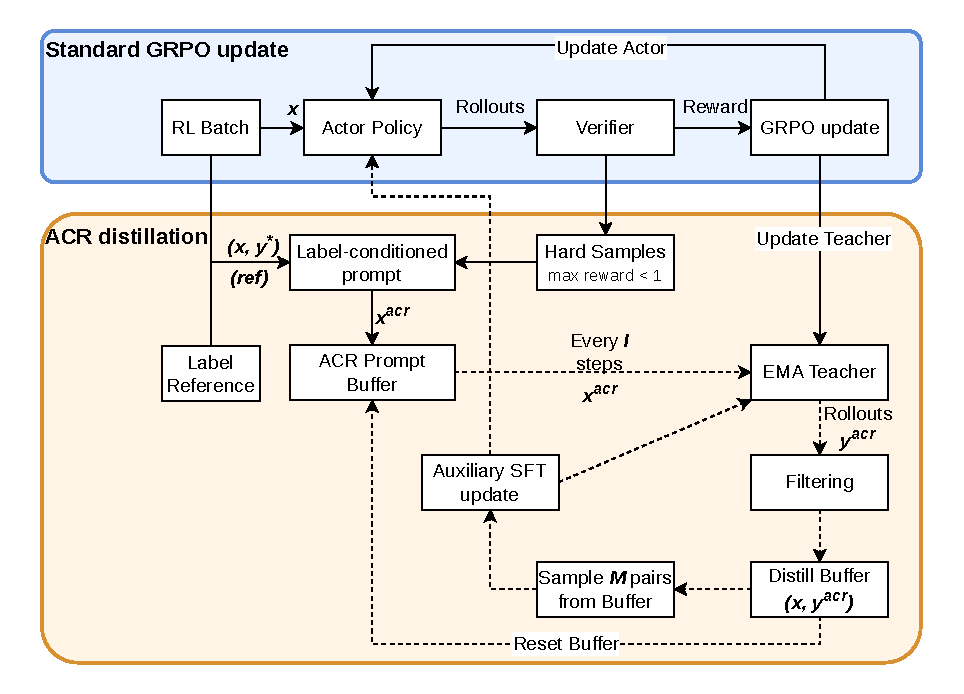
\includegraphics[width=0.85\linewidth]{figures/minerva_separated_from_original.pdf}
  \caption{MinervaRL overview separating the standard GRPO loop from the auxiliary ACR path. Solid arrows show the synchronous training flow, while dashed arrows show the periodic ACR distillation pass.}
  \label{fig:minervarl}
\end{figure}

MinervaRL augments the standard GRPO-based RLVR loop with hardness-gated answer-conditioned self-training. The central idea is simple: when the current policy cannot solve a prompt within the available rollout budget, we temporarily reveal the ground-truth label during training to elicit a short rationale that justifies it. We call the resulting trace an \emph{answer-conditioned rationale} (ACR). Importantly, the label-revealing prompt is used only to generate candidate training traces. Before distillation, each candidate is checked by the task verifier and filtered for leakage and rationale quality. Accepted traces are then distilled back into the actor using the original task prompt, without any label hint. Thus, MinervaRL uses labels to construct additional verified supervision during training, but all reported evaluations use the same answer-free prompts as the GRPO baseline.

The procedure runs on two coupled timescales. At every training step, the actor performs the ordinary on-policy GRPO update on verifier-scored rollouts from the original prompts, so the primary RLVR objective is unchanged. In parallel, MinervaRL identifies hard prompts whose rollout group contains no fully verified completion, i.e., prompts with maximum verifier reward below $1$. These prompts are added to an ACR buffer $\mathcal{P}$ together with a label-conditioned generation prompt. Every $I$ steps, an exponential moving average (EMA) teacher samples ACR candidates for the buffered prompts. Candidates that are verifier-correct and pass the filtering pipeline are stored in a distillation buffer $\mathcal{Q}$ as pairs of the original prompt and the accepted trace. The actor then receives a lightweight supervised update on samples from $\mathcal{Q}$, after which the buffers are reset. In this way, MinervaRL preserves on-policy RLVR as the main training signal while periodically converting otherwise signal-poor hard prompts into verified original-prompt training examples.































\paragraph{Notation.}
Let $\mathcal{D}=\{(x_i,y_i^\star)\}_{i=1}^{n}$ be the Minerva-CTI training set, where $x_i\in\mathcal{X}$ is the original answer-free prompt and $y_i^\star\in\mathcal{A}$ is the ground-truth structured target. The actor $\pi_\theta$ and EMA teacher $\pi_\phi$ both generate output sequences $y\in\mathcal{Y}$, including ordinary RLVR responses and ACR traces. The buffers $\mathcal{P}$ and $\mathcal{Q}$ store ACR-generation prompts and accepted original-prompt distillation pairs, respectively. We write $x_i\oplus b(y_i^\star,d_i)$ for concatenating $x_i$ with a label-conditioned ACR suffix $b(\cdot)$, where $d_i$ denotes optional canonical reference details, and $\mathrm{task}(x_i)$ for the task type of prompt $x_i$.

\paragraph{Step 1 (\Cref{alg:minervarl}): RLVR rollouts and GRPO update.}
At step $t$, we sample a batch $\mathcal{B}_t\subset\mathcal{D}$. For each $(x_i,y_i^\star)\in\mathcal{B}_t$, the actor samples $N=8$ completions from the original prompt,
\begin{equation}
    y_{i,j}^{\mathrm{rlvr}} \sim \pi_\theta(\cdot\mid x_i),
    \qquad j=1,\ldots,N ,
\end{equation}
which are scored by the verifier:
\begin{equation}
    r_{i,j}^{\mathrm{base}}
    =
    R_{\textsc{minerva}}\!\left(x_i,y_{i,j}^{\mathrm{rlvr}},y_i^\star\right).
\end{equation}
The actor is updated with GRPO using only these on-policy, original-prompt trajectories, matching the standard GRPO baseline.






\begin{algorithm}[t]
\refstepcounter{algorithm}
\label{alg:minervarl}
\centering
\begin{minipage}{0.93\linewidth}
\noindent\makebox[\linewidth][l]{\rule{0.86\linewidth}{0.8pt}}\par
\vspace{2pt}
{\normalsize\textbf{Algorithm~\thealgorithm} MinervaRL}\par
\vspace{2pt}
\noindent\makebox[\linewidth][l]{\rule{0.86\linewidth}{0.4pt}}\par
\vspace{3pt}
\footnotesize
\begin{algorithmic}[1]
\REQUIRE $\mathcal{D}=\{(x_i,y_i^\star)\}_{i=1}^{n}$; actor $\pi_\theta$; verifier $R_{\textsc{minerva}}$; RLVR rollouts $N$; ACR rollouts $K$; interval $I$; EMA decay $\alpha$; distill cap $M$; threshold $\tau_q$; SFT scale $\gamma$
\ENSURE Trained actor $\pi_\theta$
\STATE \textbf{Initialize:} $\phi\gets\theta$; $\mathcal{P},\mathcal{Q}\gets\emptyset$
\FOR{training step $t=1,2,\ldots$}
  \STATE \textbf{Step 1: RLVR rollouts and GRPO update}
  \STATE $\mathcal{B}_t\gets\textsc{SampleBatch}(\mathcal{D})$
  \FORALL{$(x_i,y_i^\star)\in\mathcal{B}_t$}
    \STATE $Y_i^{\mathrm{rlvr}}\gets\{y_{i,j}^{\mathrm{rlvr}}\sim\pi_\theta(\cdot\mid x_i)\}_{j=1}^{N}$
    \STATE $\mathbf{r}_i^{\mathrm{base}}\gets\{r_{i,j}^{\mathrm{base}}=R_{\textsc{minerva}}(x_i,y_{i,j}^{\mathrm{rlvr}},y_i^\star)\}_{j=1}^{N}$
    \STATE $m_i\gets\max_j r_{i,j}^{\mathrm{base}}$
  \ENDFOR
  \STATE $\theta\gets\textsc{GRPO}\!\left(\theta,\mathcal{B}_t,\{Y_i^{\mathrm{rlvr}},\mathbf{r}_i^{\mathrm{base}}\}_{i}\right)$;\quad
  $\phi\gets\alpha\phi+(1-\alpha)\theta$

  \STATE \textbf{Step 2: Buffer hard prompts for ACR}
  \STATE $\mathcal{P}\gets\mathcal{P}\cup
  \{(x_i,\,x_i^{\mathrm{acr}},\,y_i^\star):
  (x_i,y_i^\star)\in\mathcal{B}_t,\ x_i^{\mathrm{acr}}=x_i\oplus b(y_i^\star,d_i),
  m_i<1,\ \mathrm{task}(x_i)\ne\mathrm{CVSS}\}$

  \IF{$t\bmod I=0$}
  \STATE \textbf{Step 3: ACR generation and filtering}
    \FORALL{$(x_i,x_i^{\mathrm{acr}},y_i^\star)\in\mathcal{P}$}
      \STATE $Y_i^{\mathrm{acr}}\gets\{y_{i,k}^{\mathrm{acr}}\sim\pi_\phi(\cdot\mid x_i^{\mathrm{acr}})\}_{k=1}^{K}$
      \STATE $\mathbf{q}_i\gets\{q_{i,k}=\textsc{TextCNNGood}(y_{i,k}^{\mathrm{acr}})\}_{k=1}^{K}$
      \STATE $\mathcal{E}_i\gets
      \{k:
      R_{\textsc{minerva}}(x_i,y_{i,k}^{\mathrm{acr}},y_i^\star)=1
      \wedge \mathrm{Filter}(y_{i,k}^{\mathrm{acr}})=1
      \wedge q_{i,k}\ge\tau_q\}$
      \IF{$\mathcal{E}_i\ne\emptyset$}
        \STATE $k^\star\gets\arg\max_{k\in\mathcal{E}_i}q_{i,k}$;\quad
        $\mathcal{Q}\gets\mathcal{Q}\cup\{(x_i,y_{i,k^\star}^{\mathrm{acr}})\}$
      \ENDIF
    \ENDFOR

    \STATE \textbf{Step 4: Distill accepted traces on original prompts}
    \STATE $\mathcal{S}\gets\textsc{Sample}(\mathcal{Q},M)$;\quad
    $\theta\gets\textsc{SFT}\!\left(\theta,\mathcal{S},\gamma\,\mathrm{lr}_{\mathrm{rlvr}}\right)$;\quad
    $\mathcal{P},\mathcal{Q}\gets\emptyset$
  \ENDIF
\ENDFOR
\end{algorithmic}
\vspace{2pt}
\noindent\makebox[\linewidth][l]{\rule{0.86\linewidth}{0.8pt}}\par
\end{minipage}
\end{algorithm}










\paragraph{Step 2 (\Cref{alg:minervarl}): Hard-prompt buffering.}
For each prompt, compute the best rollout reward
\begin{equation}
    m_i=\max_{j\in\{1,\ldots,N\}} r_{i,j}^{\mathrm{base}} .
\end{equation}
We call $x_i$ hard at step $t$ if $m_i<1$, i.e., none of the sampled completions is fully verified. For each hard prompt, excluding CVSS, we construct an answer-conditioned rationale prompt
\begin{equation}
    x_i^{\mathrm{acr}} = x_i \oplus b(y_i^\star,d_i),
\end{equation}
where $b(\cdot)$ reveals the gold target and asks for a short rationale, and $d_i$ optionally contains truncated canonical reference details. We add $(x_i,x_i^{\mathrm{acr}},y_i^\star)$ to the ACR buffer $\mathcal{P}$. This gate is dynamic: a prompt stops entering $\mathcal{P}$ once the actor begins producing fully verified rollouts. We exclude CVSS because its verifier already provides dense graded feedback through CVSS base-score distance, unlike long-tail identifier tasks where incorrect IDs often yield no useful signal.

\paragraph{Step 3 (\Cref{alg:minervarl}): ACR generation and filtering.}
Every $I=10$ steps, the EMA teacher samples $K=4$ ACR candidates for each buffered prompt:
\begin{equation}
    y_{i,k}^{\mathrm{acr}}
    \sim
    \pi_\phi(\cdot\mid x_i^{\mathrm{acr}}),
    \qquad k=1,\ldots,K ,
\end{equation}
using temperature $0.7$ and nucleus sampling with $p=0.9$. We retain only candidates that are verifier-correct and pass the filtering pipeline in Appendix~\ref{app:filtering}, which removes leakage, degeneration, insufficiently grounded rationales, and low-quality traces. The eligible set is
\begin{equation}
    \mathcal{E}_i
    =
    \left\{
    k :
    R_{\textsc{minerva}}\!\left(x_i,y_{i,k}^{\mathrm{acr}},y_i^\star\right)=1
    \ \wedge\
    \mathrm{Filter}\!\left(y_{i,k}^{\mathrm{acr}}\right)=1
    \ \wedge\
    q_{i,k}\ge\tau_q
    \right\},
\end{equation}
where $q_{i,k}$ is the TextCNN \textsc{good} probability and $\tau_q=0.5$. If $\mathcal{E}_i\neq\varnothing$, we select
\begin{equation}
    k^\star=\arg\max_{k\in\mathcal{E}_i} q_{i,k}
\end{equation}
and enqueue the original-prompt distillation pair $(x_i,y_{i,k^\star}^{\mathrm{acr}})$ into $\mathcal{Q}$. Keeping at most one trace per prompt per interval prevents repeated generations from dominating the supervised update.

\paragraph{Step 4 (\Cref{alg:minervarl}): Original-prompt distillation.}
At each distillation interval, we sample up to $M=256$ pairs $\mathcal{S}\subseteq\mathcal{Q}$ and apply one supervised update:
\begin{equation}
    \mathcal{L}_{\mathrm{sft}}(\theta)
    =
    -
    \mathbb{E}_{(x,y)\sim\mathcal{S}}
    \left[
    \log \pi_\theta(y\mid x)
    \right].
\end{equation}
The update uses learning rate $\gamma\cdot\mathrm{lr}_{\mathrm{rlvr}}$ with $\gamma=0.05$, after which $\mathcal{P}$ and $\mathcal{Q}$ are reset. Because distillation is performed on the original prompt $x_i$, not on $x_i^{\mathrm{acr}}$, the actor learns from verified traces without relying on label hints at inference time.
